\phantomsection
\chapter{Facial expression recognition}

\noindent After having stated the conditions and motivations of our project, we will now describe an overview of the system we will implement. A facial recognition system can roughly be summed up as classification applied to a pre-processed image. The image processing steps, especially the feature extraction part, along with commonly used classification algorithms, will be detailed further in this chapter. Next sections will be about issues raised facial expression recognition systems, and key requirements these systems have to meet in order to be considered acceptable.

\section{General structure}

\vspace{\baselineskip}
\noindent Facial expression recognition is a system enabling an automatic recognition of emotions displayed by a human face. Facial expression recognition can be image or video-based; it can also be computed real-time. Most of the time, researchers try to recognize emotions out of images of human faces. This can also be achieved real-time on video streams : While the person displays his/her emotions, the facial expression recognition system analyses the video, and detect in real-time the displayed emotion.
\newline

\noindent In both cases, facial expression recognition process is structured as in the figure~\ref{facial_expression_recognition_process}
\newline

\begin{figure}[!h]
\begin{center}
\noindent 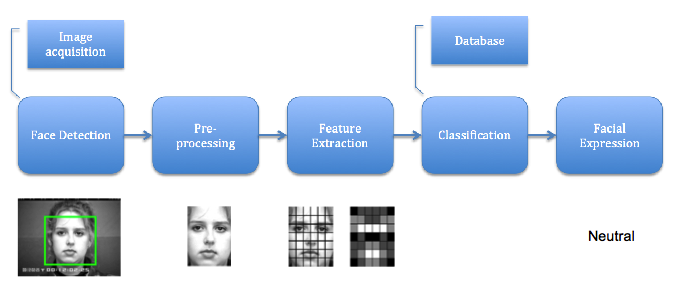
\includegraphics[scale=0.6]{figures/facial_expression_recognition_process} 
\newline
\caption{Facial Expression Recognition process}
\label{facial_expression_recognition_process}
\end{center} 
\end{figure}

\subsection{Image Acquisition}

\vspace{\baselineskip}
\noindent First step of the process is "Image Acquisition". Images used for facial expression recognition can be static images or image sequences. Image sequences give more informations about the facial expression, as the steps in muscles movement. About static images, facial expression recognition systems usually need 2D greyscale images as inputs. We can however expect future systems to use colour images; first because of the increasing affordability of technologies and devices capable of capturing images or image sequences; then because colours can give more information on emotions, i.e blushing \cite{CHI03}.
\newline

\subsection{Face Detection}

\vspace{\baselineskip}
\noindent Second step is "Face Detection". Indeed, in a static image and even more in an images sequence, this is an obvious need. Once the face has been detected, all other non-relevant information can be deleted, since only the face is needed. It could hence be included in the next step, which is "Pre-processing", but because of its importance it represents a step in itself. In a real-time facial expression recognition system working with image sequences, the face has to be detected, but also tracked. One of the most used and famous detection and tracking algorithm is the Viola-Jones Algorithm, which we will explain in detail later in this report. This algorithm can be trained to detect all kind of objects, but is mostly used for face detection. 
\newline

\subsection{Pre-processing}

\vspace{\baselineskip}
\noindent Third step is "Pre-processing", which is about applying image processing algorithms to the image, in order to prepare it for the next step. Pre-processing is usually about noise removal, normalization against the variation of pixel position or brightness, segmentation, location, or tracking of parts of the face. Emotion recognition is also sensitive to transformation, scaling and rotation of the head in the image or image sequence. In order to solve this problem, the image can be geometrically standardized. References used for this standardization are usually the eyes \cite{CHI03}.
\newline

\subsection{Features Extraction}

\vspace{\baselineskip}
\noindent Once the image has gone through the "Pre-processing" step, the next one is "Features Extraction". In this step, data is converted into a higher representation of shape, motion, colour, texture, and spatial configuration of the face or its components. One of the main goals of this step is to reduce the dimensionality of the input data. The reduction procedure should retain essential information possessing high discrimination power and high stability \cite{CHI03}. There are a lot of features extraction methods. The most famous are : Principal Component Analysis (PCA), Linear Discriminant Analysis (LDA), Problem Based Learning (PBL), Hidden Markov Models (HMM), Eigenfaces, Gabor Wavelets. The extracted data is then used in the "Classification" step.
\newline

\subsection{Classification}

\noindent The classification step marks the end of image processing steps (face detection, normalization, feature extraction). There are many kinds of classification algorithms, some of them can even be used in the feature extraction part, as stated in Section \ref{feat_x}. This step takes into input a model previously trained with pre-processed data, and test data made of feature vectors extracted from the image we want to label. Feature vectors from pre-processed data and test data have to be obtained using the same feature extraction algorithm. The chosen classifier then outputs a value corresponding to the label of the class the picture belongs to.
\vspace{\baselineskip}

\phantomsection
\section{Feature extraction algorithms} \label{feat_x}

\vspace{\baselineskip}
\noindent Before developing a facial expression recognition project, it is important to know what already exists; the state of the art of facial expression recognition system. In this chapter, an overview will be given of the existing systems before to decide on a system for the project.
\newline

\noindent 2 main categories of feature extraction algorithms can be distinguished : \textit{appearance-based} or \textit{geometry-based}. The first ones are algorithms that try to find basic vectors characterising the whole picture, usually by a dimensionality reduction method. These algorithms lead to a simplification of the dataset, while retaining the main characteristics of the picture. However, these methods have to be carefully parametrized, so they do not encounter the "curse of dimensionality", which is about processing high-dimensional data.
\vspace{\baselineskip}

\noindent Examples of appearance-based methods : Principal Component Analysis, Linear Discriminant Analysis, Hidden Markov Models, Eigenfaces
\newline

\noindent The second type of feature extraction algorithms is geometry-based algorithms. These methods tend to locate important features, and build the feature vectors depending on those regions of interest. The key point of these methods is that the face is not a global structure anymore. Indeed, it has been summarized in a set of features regions, which are themselves translated into feature vectors.
\vspace{\baselineskip}

\noindent Examples of geometry-based methods : Gabor Wavelets, Local Binary Patterns
\newline

\subsection{Principal Component Analysis (PCA)}

\vspace{\baselineskip}
\noindent This is a statistical method; one of the most used in linear algebra. PCA is mainly used to reduce high dimensionality of data and to obtain the most important information from this data. Because Facial Expression Recognition needs to reduce the dimensionality of data during features extraction, PCA is commonly used. It helps transforming high dimensionality of data to a new coordinate system of lower dimensions while still preserving the most important information. PCA computes a covariance matrix and a set of values called the eigenvalues and eigenvectors from the original data \cite{GAN08}. Since it is a statistical method, it can also be used in the classification step.
\newline

\subsection{Linear Discriminant Analysis (LDA)}

\vspace{\baselineskip}
\noindent Linear Discriminant Analysis is also a statistical method, used to classify a set of objects into groups. It is done by observing a set of features that describe the objects. LDA as PCA are used to establish a linear relationship between the dimensions of the data. The main difference is that LDA uses the linear relationship to model the differences into classes of objects and PCA does not take any differences into account in the linear relationship. The idea is to perform a linear transformation on the data to obtain a lower dimensional set of features \cite{GAN08}. Like PCA, LDA is also a classification algorithm.
\newline

\subsection{Local Binary Patterns (LBP)}

\vspace{\baselineskip}
\noindent This is an appearance-based method. It can be used to describe texture and shape. LBP extracts some informations from the neighbourhood of a central pixel. It compares the intensity values of the neighbourhood pixels with the intensity value of the central pixel  \cite{GAN08}. This method is the one that will be used for this Facial Expression Recognition system.
\newline

\subsection{Hidden Markov Models (HMM)}

\vspace{\baselineskip}
\noindent These models are a set of statistical models used to characterize the statistical properties of a signal \cite{RAB93}. It can be used as a classification algorithm, and canalso be  developed to recognize expressions based on the maximum likelihood decision criterion \cite{LIE98}.
\newline

\subsection{Eigenfaces}

\vspace{\baselineskip}
\noindent Eigenfaces are a set of eigenvectors which are derived from the covariance matrix of a set of face images in a high-dimensional vector space. The eigenvectors are ordered and each one represents the different amount of the variation among the face images. It all together characterizes the variation between face images \cite{TUR91}.
\newline

\subsection{Gabor Filters}

\vspace{\baselineskip}
\noindent Gabor filters are applied in order to extract a set of Gabor wavelet coefficients. When convolving these Gabor filters with a simple face image, filter responses are obtained. These representations display desirable locality and orientation performance \cite{JEM09}. However, it has a limitation which is the processing time of Gabor feature extraction. It is very long and its dimension is prohibitively large \cite{PRA09}.
\newline

\phantomsection
\section{Issues}

\vspace{\baselineskip}
\subsection{Database}

\vspace{\baselineskip}
\noindent Databases can be a source of issues. As said previously, databases should fulfill a number of requirements in order to be the most efficient as possible. 
\newline

\noindent If the Facial Expression Recognition system wants to be close to reality, it should be able to recognize spontaneous expressions rather than posed expressions. Indeed, spontaneous expressions are closer to reality than posed expressions. Posed expressions are exaggerated. While creating a database of spontaneous expressions, Sebe and colleagues \cite{SEB07} made some observations of the major problems they encountered \cite{BET12}:
\newline
\begin{itemize}
  \item Different subjects express the same emotions at different intensities
  \item If the subject becomes aware that he or she is being photographed, their expression loses its authenticity
  \item Even if the subject is not aware of the recording, the laboratory conditions may not encourage the subject to display spontaneous expressions.
\end{itemize}

\vspace{\baselineskip}
\noindent In order to get round of these problems, they came up with a method. The method was to record facial expressions with a camera hidden in a video kiosk. The video kiosk was displaying emotion inducing videos. Once the recording was done, subjects were notified of the recording and were asked for their permission to use the captured images and videos for research studies. Then the subjects explained which emotions they felt and expressed and their replies were documented against the recordings of the facial expressions \cite{SEB07}.
\newline

\noindent They found that a wide range of expressions are hard to induce and particularly fear and sadness. They also found that spontaneous expressions could be misleading: some subjects express one emotion while feeling another one (for example, one subject was showing sadness while being happy) \cite{SEB07}.
\newline

\noindent At the end, databases bring some issues that can affect the authenticity of the recognition system. It depends of the type of the expressions : spontaneous or posed expressions. If the system aims to recognize facial expressions of people unaware of it, spontaneous expressions databases will be used but it leads to authenticity issues as seen previously. If the system aims to recognize facial expressions of people asked to express certain emotion, posed expressions databases will be used but the result will not be close to the reality.
\newline

\subsection{Real-time}

\vspace{\baselineskip}
\noindent The goal of the Facial Expression Recognition system of this paper is to recognize facial expression in real time. For a real-time application, the processing should not be too heavy otherwise the time of processing will be too long and the application will not be in real time anymore. 
\newline

\noindent This is one of the challenges of this kind of system. Because most of the time the processing is really heavy whatever the algorithm is and it is really difficult to make it work in real-time. Most of the applications in need of Facial Fxpression Recognition are in need of real-time recognition. For example in robotics, or in surveillance. The solution could be to find new algorithms for Facial Expression Recognition or to improve and lighten already existing algorithms.
\newline

\subsection{Conditions}

\vspace{\baselineskip}
\noindent Another one of the challenges of this kind of system is to be independent to the conditions of the recording. It means that the recognition should not be disturbed by occlusions for example, or difference in the lighting, or even by the angle that the face makes with the camera lens. This examples cover almost all the conditions that can change during the recording and have an influence on the recognition system. 
\newline

\subsubsection{Occlusion}

\vspace{\baselineskip}
\noindent "Occlusion" represents all the elements that can cover the face or a part of it. For example, a beard, a scarf masking the bottom of the face, glasses or bangs. By hiding a part of the face, these occlusions can affect the recognition. Indeed, these Facial Expression Recognition systems are based on comparison of features and if all the features cannot be compared because something is covering a part of the face, the recognition is affected. In order to compensate for this problem, some databases includes data with already occlusions in it as beard, glasses or scarf for example. This is the case for the AR Face database and some examples of the images contained in this database are given by figure~\ref{arface_example2} and figure~\ref{arface_example3} \cite{ARFACE}:
\newline

\begin{figure}[!h]
\begin{center}
\noindent 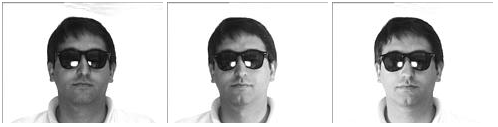
\includegraphics[scale=0.7]{figures/arface_example2} 
\newline
\caption{example of occlusion by sunglasses in the AR Face database}
\label{arface_example2}
\end{center} 
\end{figure}

\begin{figure}[!h]
\begin{center}
\noindent 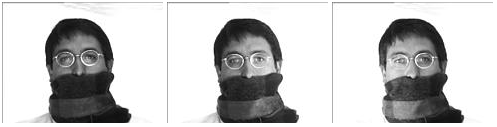
\includegraphics[scale=0.7]{figures/arface_example3} 
\newline
\caption{example of occlusion by scarf and glasses in the AR Face database}
\label{arface_example3}
\end{center} 
\end{figure} 

\subsubsection{Lightning}

\vspace{\baselineskip}
\noindent As for occlusion, lightning is an element that can affect Facial Expression Recognition system. With a lightning different from the one used in the database, the recognition will be less efficient. All the conditions that change from the one of the database on which is based the recognition process will disturb the recognition in itself. If the images are brighter or darker than the one of the database, some details can disappear or some features cannot be recognized as well as if the conditions were the same. In order to compensate for this problem, some databases includes data with already changes in the lightning. This is the case for the AR Face database and an example of the images contained in this database is given by the figure~\ref{arface_example1} \cite{ARFACE}:
\newline

\begin{figure}[!h]
\begin{center}
\noindent 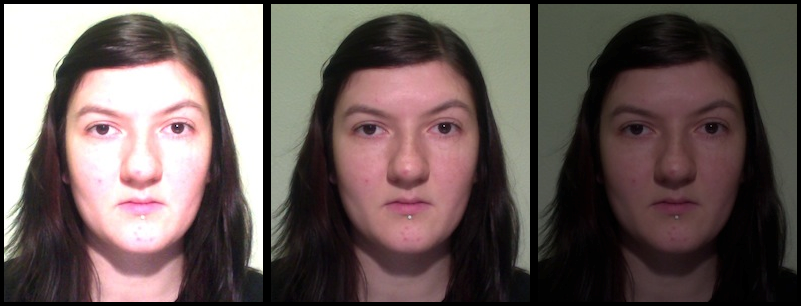
\includegraphics[scale=0.7]{figures/arface_example1} 
\newline
\caption{example of different lightnings (from left to right: dark to bright) in the AR Face database}
\label{arface_example1}
\end{center} 
\end{figure}

\subsubsection{Angle}

\vspace{\baselineskip}
\noindent The angle of the head from the camera lens is one of the conditions that can affect the most the recognition process. Indeed if the head is too much turned from straight angle, some features will disappear. For example, with a profile angle, one eyes and half of the nose and of the mouth disappear. And if the database does not contain sample with profile face, the recognition will not succeed. This constraint is based on the database; if the database contains images from straight angle as well as from profile angle and other, the recognition will be possible even if the head is not with a straight angle. But if the database contains images only from straight angle, the recognition will be almost impossible if the head is turned. An example of the different images taken from different angles for one emotion, "Fear", from the KDEF database is given in figure~\ref{kdef_example_angle}:
\newline

\begin{figure}[!h]
\begin{center}
\noindent 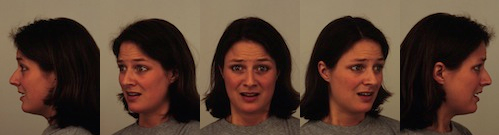
\includegraphics[scale=0.8]{figures/kdef_example_angle} 
\newline
\caption{example of different angles of the "Fear" emotion (from left to right: full left profile, half left profile, straight, half right profile, full right profile) in the KDEF database}
\label{kdef_example_angle}
\end{center} 
\end{figure}

\phantomsection
\section{Requirements}

\vspace{\baselineskip}
\noindent Based on everything that was said previously, the Facial Exression Recognition system of this paper can be defined by some requirements. Additional requirements may be defined further in this paper. Here are the requirements already defined :
\newline

\begin{itemize}
  \item Able to recognize basic emotions : 
  \noindent As explained before, Facial Expression Recognition systems are able to recognize 6 basic emotions and the neutral state. This system would be able to do the same: recognize the 6 basic emotion that are "Happiness", "Fear", "Surprise", "Disgust", "Sadness", "Anger" and the neutral state.
\newline

  \item Able to work in real-time : 
  \noindent This system would be able to recognize emotion in real-time. It means that it could recognize expressions based on a video sequences . It also means that the algorithm for the feature extraction could not have heavy processing or to use one that would be lightened. 
\newline

  \item Recognition from straight angle of the face : 
  \noindent This system would be able to recognize facial expression from a straight angle of the face. It means that the system would be able to detect faces that are in front of the camera lens and to recognize expressions in these faces. It would not be able to recognize emotions on a face that is from profile or half-profile.
\newline

  \item Recognition with no occlusion on the face : 
  \noindent This system would be able to recognize emotions with no occlusion on the subject's face. It means that the face would not be cover in any way: no glasses, no beard or no scarf. The face would be complete and not masked.
\newline

  \item Recognition with no change in lightning : 
  \noindent This system would be able to recognize emotions on faces under the same lighting conditions. It means that the light would not vary during the recognition part. The light would stay the same and the level of intensity of the light would be as close as possible that the one of the database. This way the lightning would not have any influence on the recognition.
\newline
\end{itemize}











